%\begin{itemize}
%	\item We show performance on the ``big tasks''(TIMIT, yearpred, CovType, Census, Adult).
%	\item We explain these results in terms of the ``small tasks'' (Census and Subsampled CovType), where we measure $\Delta$, showing that below a certain number of bits, $\Delta$ can increase a lot.  If we have space, we explain the trade-offs here a bit, showing in the fixed design setting that higher noise means higher $\lambda^*$, which means fewer bits can be used until $\Delta$ increases a lot.
%	\item We briefly present low-precision training, showing that performance doesn't degrade much relative to full-precision training.
%\end{itemize}
In this section, we empirically evaluate our generalization theory on low-precision RFF, and demonstrate the empirical generalization performance of low-precision RFF under memory budgets. On the Census dataset and subsampled Covtype, we first demonstrate the strong correlation of generalization performance and $\Delta$, which aligns with our $\Delta$ based bounds of generalization bound for low-precision RFF. We then extend to four different datasets, including the Census, YearPred dataset for kernel ridge regression and the Covtype, TIMIT dataset for kernel logistic regression. \todo{Jian describe how the memory is calculated}

\subsection{Strong correlation between generalization and $\Delta$\todo{Jian: need a english name for $\Delta$}}
Our theory in Section~\ref{sec:lprff} claims that in fixed design kernel ridge regression, the generalization performance strongly depends on the quantity $\Delta$.
To validate the strong correlation between generalization performance and the central quantity $\Delta$ in our generalization bound, we empirically show that the number of bits generating smaller $\Delta$ demonstrates better generalization performance. 
Specifically, we analyze the correlation on the Census dataset for kernel ridge regression. In addition, we demonstrate that this correlation from kernel ridge regression theory empirically generalize to kernel logistic regression. 

We solve the regression problem with closed form solution. In our experiment, we grid search the best-performing regularizer strength for the exact kernel; this best-performing regularizer strength is uniformly applied to all the different runs. For kernel logistic regression, we subsample 20k data points for both training and heldout set of the Covtype dataset to tractably compute $\Delta$. As there is no closed-form solution for logistic regression, we train with SGD using minibatch 250. We grid search the best performing learning rate and regularizer strength using 20k dimensional \Nystrom approximation as proxy to the optimal values for the exact kernel; the 20k dimensional \Nystrom approximation and the exact kernel share the same training kernel matrix. We grid search the regularizer strength from grid $\{1e^{-5}, 5e^{-5}, 1e^{-4}, 1e^{-3}, 5e^{-3}, 1e^{-2}, 5e^{-2}, 1e^{-1}\}$ for both task. The learning rate in logistic regression experiment is from the grid $\{5, 10, 50, 100\}$. We report the average $\Delta$ and the average generalization performance, along with the standard deviation, from 5 different random seeds.

In Figure~\ref{fig:generalizatio_col}, we can observe LP-RFF can achieve significantly smaller $\Delta$ and generalization performance than full precision RFF and \Nystrom. Specifically, 8 bits and 2 bit LP-RFF attains the optimal generalization performance for Census and Covtype respectively. Noticeably, on both the Census and the Covtype dataset, approximation configurations which have low $\Delta$ value also shows better generalization performance. The ordering with respect to $\Delta$ aligns well with the one with respect to generalization performance, demonstrating a strong correlation between $\Delta$ and generalization performance for approximated kernels.

\begin{figure}
	\centering
	\begin{tabular}{c c c c}
		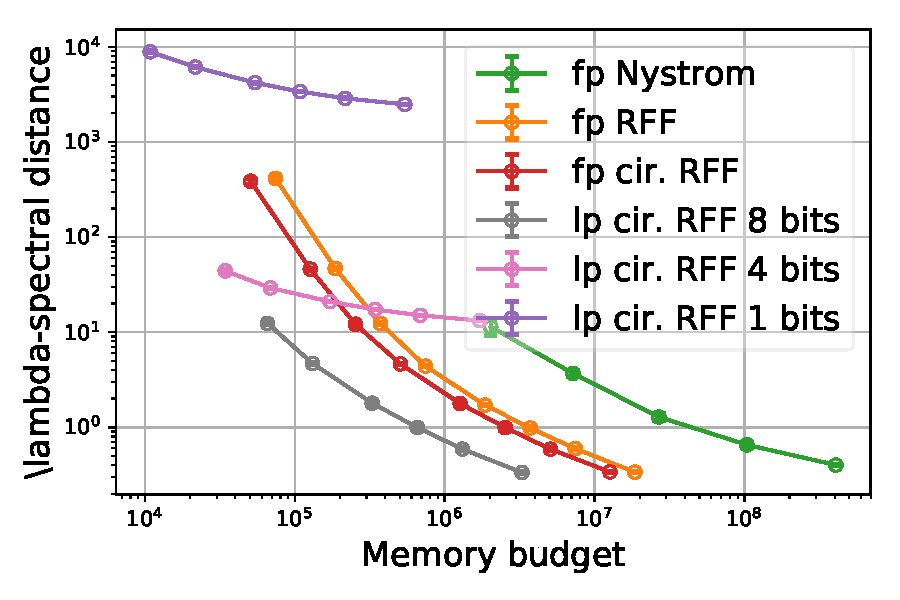
\includegraphics[width=0.24\linewidth]{figures/regression_delta_vs_mem.pdf} &
		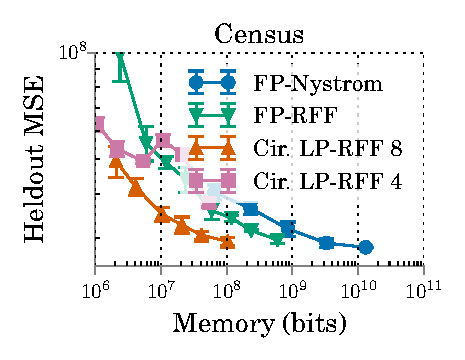
\includegraphics[width=0.24\linewidth]{figures/regression_l2_vs_mem.pdf} &
		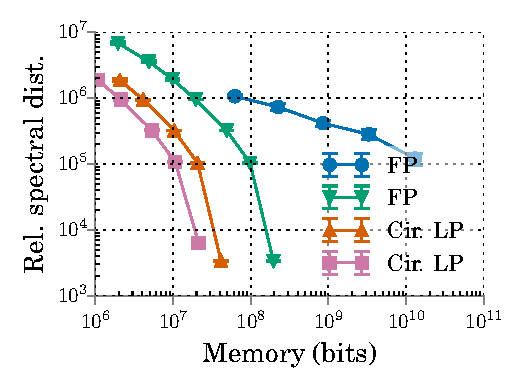
\includegraphics[width=0.24\linewidth]{figures/classification_delta_vs_mem.pdf} &
		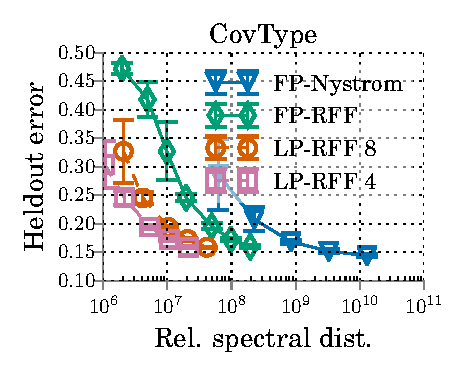
\includegraphics[width=0.24\linewidth]{figures/classification_acc_vs_mem.pdf} 
	\end{tabular}
	\caption{The strong correlation between generalization performance and $\Delta$ under memory budgets. Under different memory budget, the precision demonstrates smaller $\Delta$ tends to have better generalization performance.}
	\label{fig:generalizatio_col}
\end{figure}


\subsection{Generalization performance of low-precision random Fourier features}
\begin{figure}
	\centering
	\begin{tabular}{c c c c}
		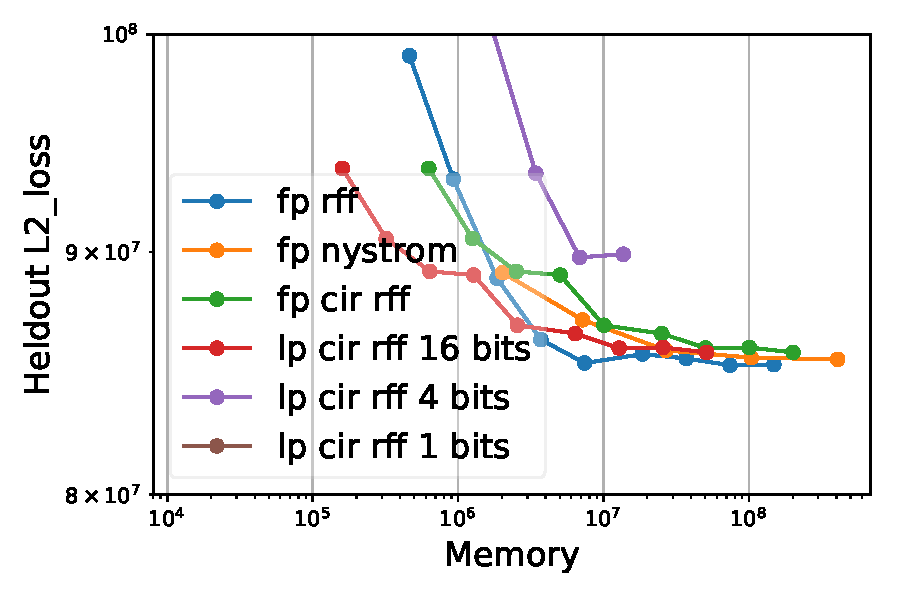
\includegraphics[width=0.24\linewidth]{figures/census_L2_loss_vs_n_memory.pdf} &
		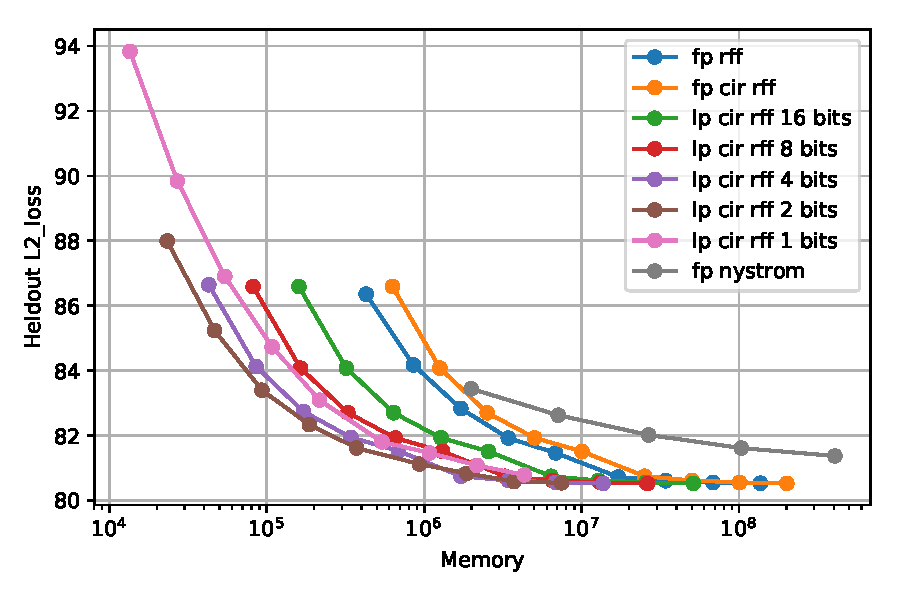
\includegraphics[width=0.24\linewidth]{figures/yearpred_L2_loss_vs_n_memory.pdf} &
		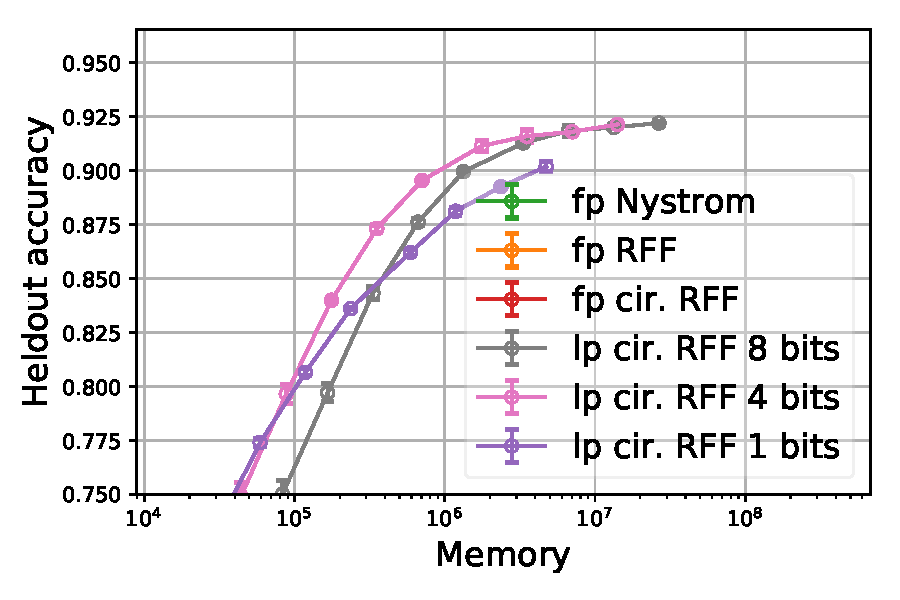
\includegraphics[width=0.24\linewidth]{figures/covtype_accuracy_vs_n_memory.pdf} &
		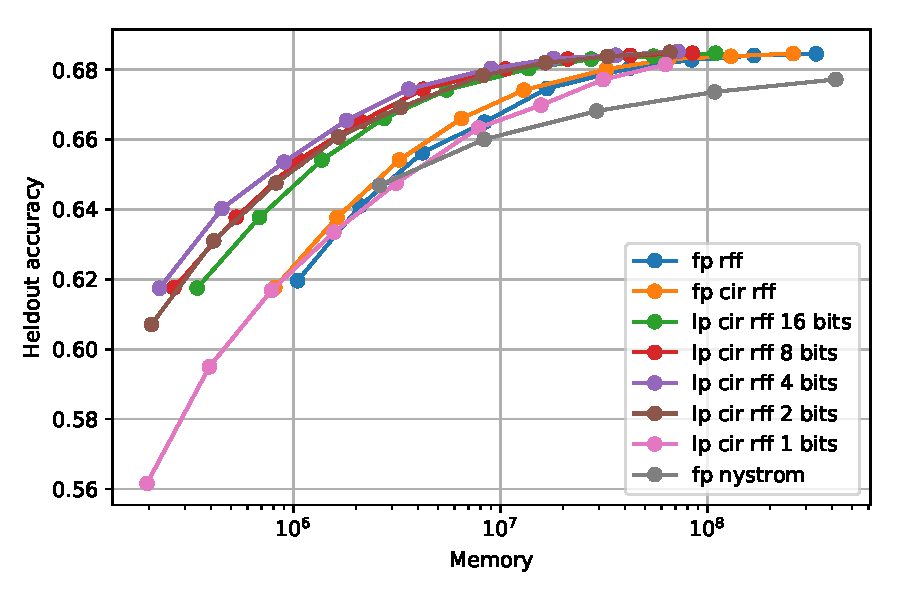
\includegraphics[width=0.24\linewidth]{figures/timit_accuracy_vs_n_memory.pdf} \\
		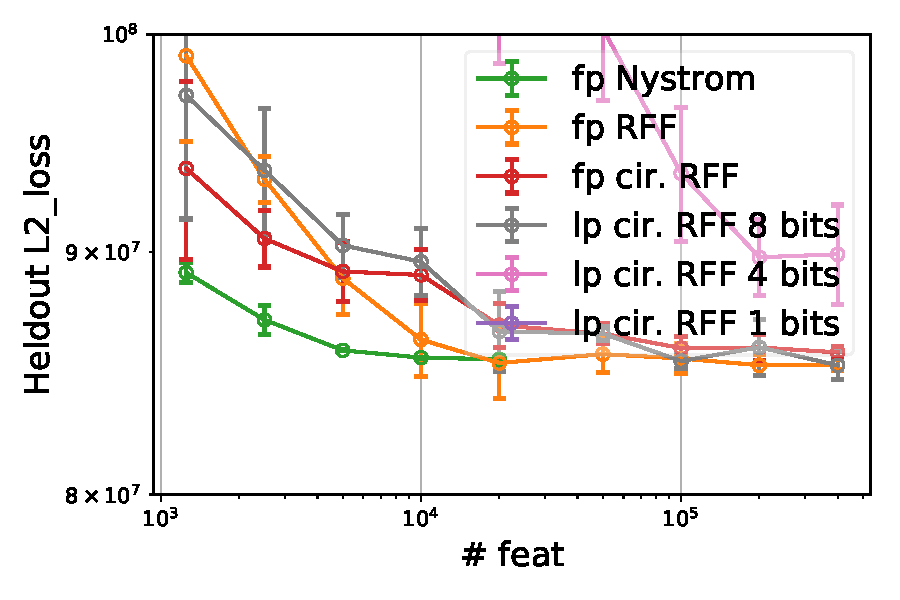
\includegraphics[width=0.24\linewidth]{figures/census_L2_loss_vs_n_feat.pdf} &
		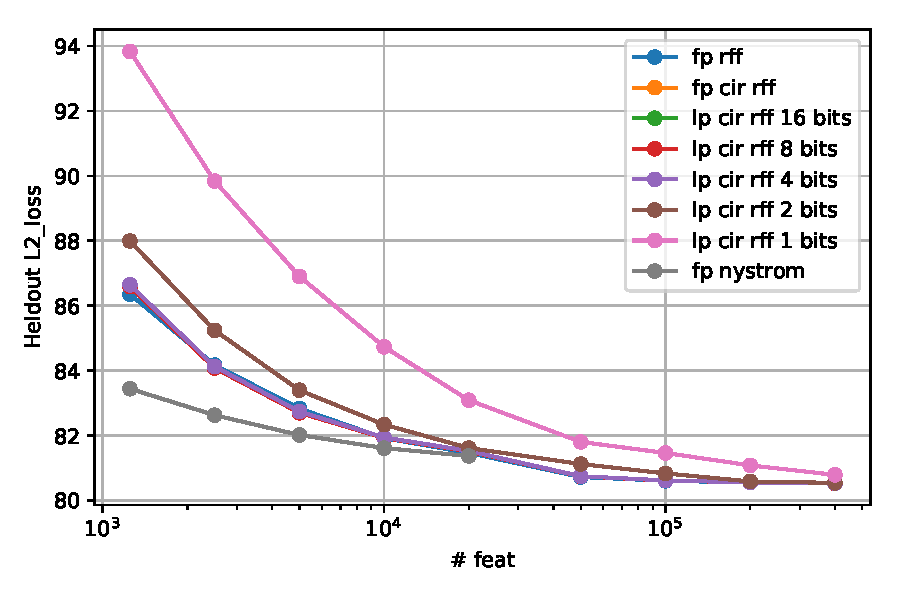
\includegraphics[width=0.24\linewidth]{figures/yearpred_L2_loss_vs_n_feat.pdf} &
		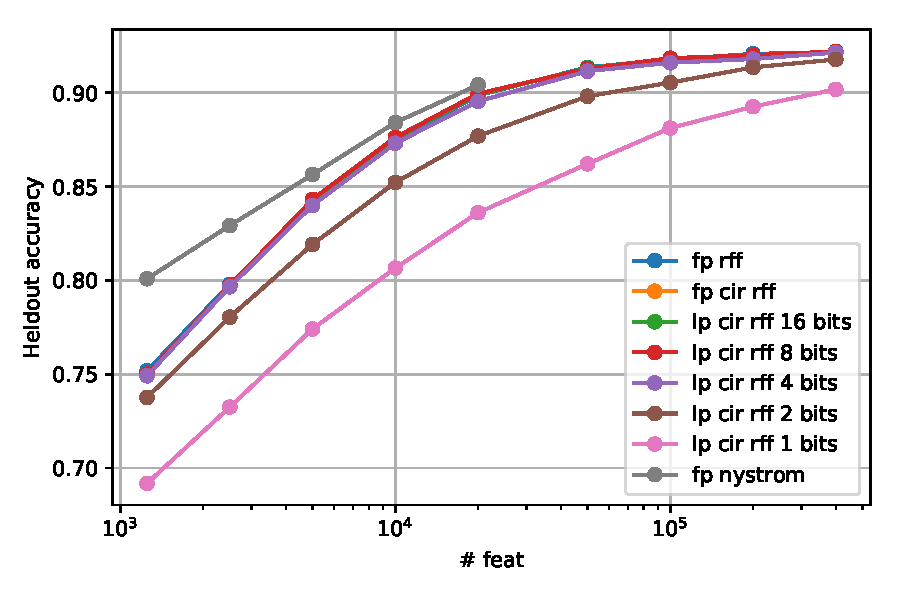
\includegraphics[width=0.24\linewidth]{figures/covtype_accuracy_vs_n_feat.pdf} &
		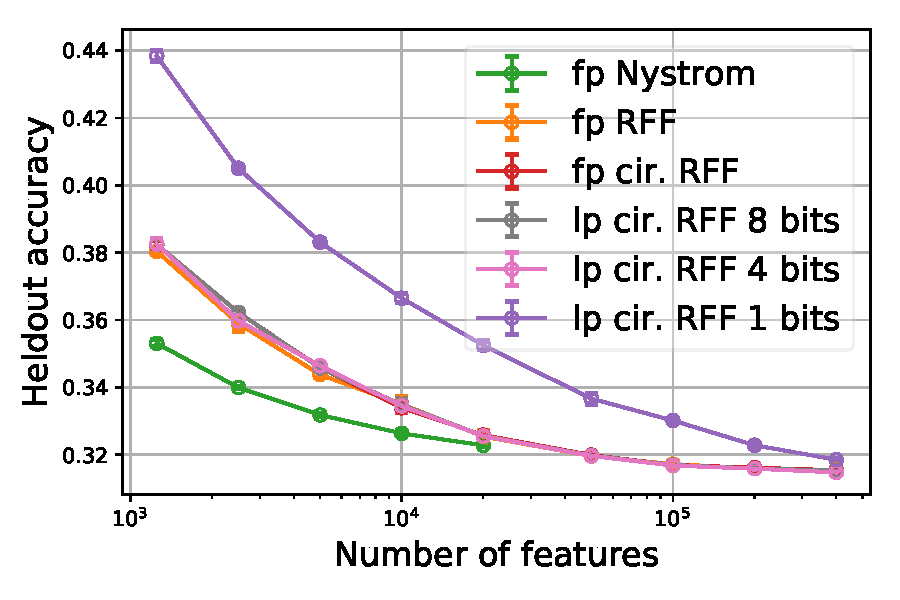
\includegraphics[width=0.24\linewidth]{figures/timit_accuracy_vs_n_feat.pdf} \\
		(a) Census & (b) YearPred & (c) Covtype & (d) TIMIT \\
	\end{tabular}
	\caption{Generalization performance of low precision RFF, full precision RFF and \Nystrom with respect to number of features and memory budgets.}
	\label{fig:generalizatio_col}
\end{figure}


\begin{figure}
	\centering
	\begin{tabular}{c c c c}
		\hline
		& FP RFF & FP circulant RFF & \Nystrom \\
		\hline
		\hline
		Census & 5.56x & 30.32x & 122.52x \\
		YearPred & 19.35x & 14.30x & 829.15x \\ 
		Covtype & 9.17x & 7.57x & 460.80x \\ 
		TIMIT & 70.42x & 25.68x & 843.41x \\ 
		\hline
	\end{tabular}
	\caption{The memory savings from LP RFF to achieve within $1e^{-4}$ relative difference from the best generalization performance of baselines. We measure heldout L2 loss and heldout accuracy as the generalization performance respectively for regression and classification problems.}
	\label{fig:mem_saving}
\end{figure}